% =====================================================================================
%  AudioPIN -- course project report (IEEE conference template, IEEEtran)
%  Limit: 4 pages excluding references. Do not change fonts, margins or spacing.
%
%  Tables II and III (pilot) are inline below; numbers from the lock-app logs and the SUS form.
% =====================================================================================
\documentclass[conference]{IEEEtran}

\usepackage{cite}
\usepackage{amsmath,amssymb}
\usepackage{graphicx}
\usepackage{booktabs}
\usepackage{url}
\usepackage{xcolor}

% Placeholder for numbers that only the pilot study can give. Delete the macro use once filled.
\newcommand{\tbd}[1]{\textcolor{red}{[#1]}}

\begin{document}

\title{AudioPIN: Observation-Resistant PIN Entry\\with One-Time Spatial-Audio Keys}

\author{
\IEEEauthorblockN{Juhi Chaudhary}
\IEEEauthorblockA{{P25CS0005}\\Department of Computer Science and Engineering\\{Indian Institute of Technology, Jodhpur}\\{p25cs0005@iitj.ac.in}}
\and
\IEEEauthorblockN{{Ranvir Kumar Singh}}
\IEEEauthorblockA{{P25CS0007}\\Department of Computer Science and Engineering\\{Indian Institute of Technology, Jodhpur}\\{p25cs0007@iitj.ac.in}}
}

\maketitle

% ------------------------------------------------------------------------------------- abstract
\begin{abstract}
A PIN typed in public is easy to watch and to record. AudioPIN keeps the PIN off the screen. For every
digit, the user's earphones play one short spatial sound whose identity and direction encode a fresh
random key from 0 to 9, read from a public chart; the user taps the digit plus the key, modulo ten.
Because the key is uniform and new for every digit of every login, each tap is equally likely, and video
of any number of logins reveals nothing. A Bayes-optimal attack simulation over five direction layouts
shows that a video-only attacker stays at chance (0.03\%), while one whose microphone identifies the
sounds breaks 0.5--18.8\% of PINs after one login. In a pilot with our lock app, successful unlocks took
a median of 15.0\,s, but only 11 of 35 attempts succeeded; the SUS score averaged 70.5.
\end{abstract}

\begin{IEEEkeywords}
authentication, shoulder surfing, PIN entry, spatial audio, HRTF, usable security
\end{IEEEkeywords}

% ------------------------------------------------------------------------------------- I
\section{Introduction}
A four-digit PIN still guards most phones, banking apps and payment cards, and it is entered in buses,
offices and queues where other people can see the screen. A single glance can be enough to learn it,
and a hidden or phone camera removes even the need to be close. The weakness is structural: the digits
the user taps \emph{are} the secret, so anyone who sees the taps sees the PIN.

Our idea is to separate what the user taps from what the user knows. Almost everyone already carries a
private output channel, a pair of earphones, and we use it to deliver a one-time key for every digit.
The screen shows only a public chart and a ring of numbers; the key arrives as a sound whose identity
and direction only the wearer can perceive. Naitou et al.~\cite{naitou2026audiopin} recently proposed a
spatial-audio scheme under the same name, in which the secret is itself a sequence of sounds selected by
turning the head. Our design differs in that the secret stays an ordinary numeric PIN, entry needs no
head tracking, and the security claim is stated and tested rather than assumed.

The objectives of this work are to:
\begin{itemize}
\item design PIN entry in which the user never waits for a particular cue, unlike earlier audio and
haptic schemes;
\item give a simple, provable property: taps carry no information about the PIN, however many
logins are recorded;
\item measure, for the first time on a spatial-audio scheme, how an attacker who also records sound
fares, and how this depends on the direction layout; and
\item choose cue sounds by their shape over time, not only by pitch, so that they remain easy to place.
\end{itemize}

% ------------------------------------------------------------------------------------- II
\section{Related Work}
\textbf{Cognitive and challenge--response entry.} Roth et al.~\cite{roth2004pin} introduced cognitive
trapdoor games, in which the user answers rounds of coloured keypads; a full recording of one
session breaks the deterministic version. SSSL~\cite{perkovic2010sssl} sends a secret challenge digit
over earphones and the user answers on a public keypad, taking about 8\,s for a five-digit PIN.
Perkovi\'c et al.~\cite{perkovic2010partially} also showed that response \emph{timing} can leak the
secret in such schemes, a point we return to in Section~\ref{sec:results}.

\textbf{Audio and haptic cues.} The Phone Lock~\cite{bianchi2011phonelock} and
Spinlock~\cite{bianchi2011spinlock} deliver cues through sound or vibration and ask the user to wait for,
or count, the right one before tapping. Security comes from the observer not knowing when the right cue
arrived, but the user pays for it in waiting time. Our wait-for-cue baseline implements this style.

\textbf{Visible randomisation.} SwiPIN~\cite{vonzezschwitz2015swipin} maps digits to swipe gestures
that change after every input and averages 3.7\,s per entry. It resists a human watching once, but the
mapping is shown on screen, so a video captures both mapping and gesture.

\textbf{Spatial audio.} The closest work, Naitou et al.~\cite{naitou2026audiopin}, places sounds around
the head and lets the user select their secret sounds by turning towards them. Twenty participants
reached 91.0\% success at 20.6\,s in the best arrangement. The paper does not evaluate an attacker,
compare against a normal PIN, or test whether users can remember a self-chosen secret. Generic
head-related transfer functions (HRTFs), as used by browsers, are known to cause front--back
confusions~\cite{wenzel1993localization,wightman1999frontback}; we turn this into a design parameter.

% ------------------------------------------------------------------------------------- III
\section{Proposed Approach}
\subsection{Threat model}
The attacker can watch the screen and the user's hand, directly or on video, for as many logins as they
like, and may place a microphone near the user. The device itself is not compromised. The user wears
stereo earphones; phone-speaker playback, a single bud or the \emph{Mono Audio} setting would remove
direction for the user and expose the sound, so the lock app begins with a left/right earphone check.

\subsection{Key-code entry}
For each PIN digit $d\in\{0,\dots,9\}$ and a layout with $n$ directions, the device draws a fresh key
and encodes it as a sound row $r$ and a direction column $c$ of the public chart:
\begin{equation}
k \sim \mathcal{U}\{0,\dots,9\},\qquad r=\left\lfloor k/n \right\rfloor,\qquad c = k \bmod n .
\label{eq:key}
\end{equation}
After a 250--300\,ms pause the cue plays. The user reads its number off the chart, counts that many
steps clockwise from their digit on a ring of 0--9, and taps $t=(d+k)\bmod 10$. The device recovers
$d=(t-k)\bmod 10$ and checks the full PIN only at the end, so a wrong entry never says which digit
failed. If no tap arrives, the \emph{same} cue repeats 2\,s after it ends. Since $k$ is uniform and
independent of $d$,
\begin{equation}
\Pr[t \mid d] = \tfrac{1}{10}\quad\text{for every } d,
\label{eq:uniform}
\end{equation}
so observed taps, from one login or many, carry no information about the PIN. For example, PIN
2\,7\,0\,5 with keys 3\,9\,1\,4 is entered as 5\,6\,1\,9; the next login, with keys 7\,2\,8\,0, as
9\,9\,8\,5. Fig.~\ref{fig:screen} shows the entry screen.

\begin{figure}[t]
\centering
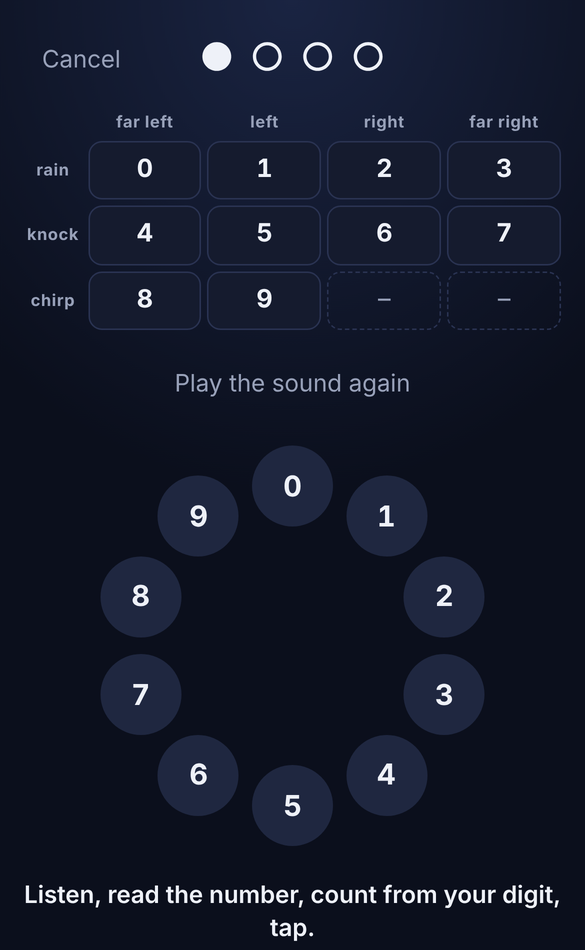
\includegraphics[width=0.46\columnwidth]{figures/entry_screen.png}
\caption{Key-code entry with four side positions and three sounds. The chart is public; nothing on
screen shows which cue played.}
\label{fig:screen}
\end{figure}

\subsection{Layouts and sound design}
A layout with $n$ directions needs $\lceil 10/n\rceil$ sounds. We support five layouts, from two
directions with five sounds to five directions with two sounds (Table~\ref{tab:attack}); only these two
extremes fill the chart exactly. The choice matters because a microphone can pick up \emph{which} sound
played far more easily than \emph{where} it seemed to come from.

Sounds are placed with the browser's HRTF panner, which works through level and time differences
between the ears. Measured on our renderer, a source at the left versus the right differs by about
12\,dB and 0.75\,ms, whereas front and back reach the two ears with 0.0\,dB and 0.000\,ms difference,
i.e.\ identical signals. Level differences arise mainly above about 1.5\,kHz: a bass-heavy knock gave
only 2.6\,dB between the ears, and 9\,dB once brightened. We therefore chose five recordings that differ
in their envelope over time---continuous rain, a single wooden knock, short bird chirps, a ringing
cowbell and a swelling cat call---each with a sharp onset and some treble~\cite{mixkit}.

\subsection{Implementation}
AudioPIN is written in plain HTML, CSS and JavaScript and runs in any modern phone browser. A shared
audio engine folds each recording to mono, removes leading silence, keeps at most 1\,s, equalises
loudness so that volume is never a clue, and plays it through a Web Audio \texttt{PannerNode} with the
HRTF model~\cite{w3c2021webaudio}. Keys come from \texttt{crypto.getRandomValues}. The research
prototype implements the three study conditions and logs every answer to CSV. The lock app is an
installable web app that stores only a salted PBKDF2 hash of the PIN, locks for 30\,s after three
wrong PINs, and works offline. An opt-in setting can keep an encrypted copy so that users may view
their PIN; it is off by default because it trades security for convenience. Code, tests and analysis
scripts are public~\cite{audiopin2026code}.

% ------------------------------------------------------------------------------------- IV
\section{Preliminary Results}
\label{sec:results}
\subsection{Attack simulation}
We simulate a Bayes-optimal attacker on uniformly random PINs (20{,}000 per cell) who gets three
guesses. The attacker either (i) sees only the taps, (ii) also identifies the sound of every cue, after
one to three observed logins, or (iii) also hears the side of the cue, as an off-centre microphone
would, with front and back indistinguishable. Seven cases with a closed-form answer, such as exactly
$3/16$ for two directions with the sound known, match the simulation.

\begin{table}[t]
\centering
\caption{PINs broken within three guesses (\%), simulated with perfect identification. Chance is 0.03\%.}
\label{tab:attack}
\setlength{\tabcolsep}{4pt}
\begin{tabular}{lccc}
\toprule
Layout (dirs $\times$ sounds) & Video & + sound, 1/2/3 logins & + side \\
\midrule
$5\times2$                         & 0.03 & 0.5 / 5.0 / 16.4  & 37.2 \\
$4\times3$, four side positions    & 0.03 & 2.4 / 19.8 / 46.9 & 18.8 \\
$4\times3$, L/F/R/B                & 0.03 & 2.4 / 19.8 / 46.9 & 79.8 \\
$3\times4$                         & 0.03 & 7.6 / 43.1 / 74.7 & 100 \\
$2\times5$                         & 0.03 & 18.8 / 70.2 / 91.4 & 100 \\
\bottomrule
\end{tabular}
\end{table}

\begin{figure}[t]
\centering
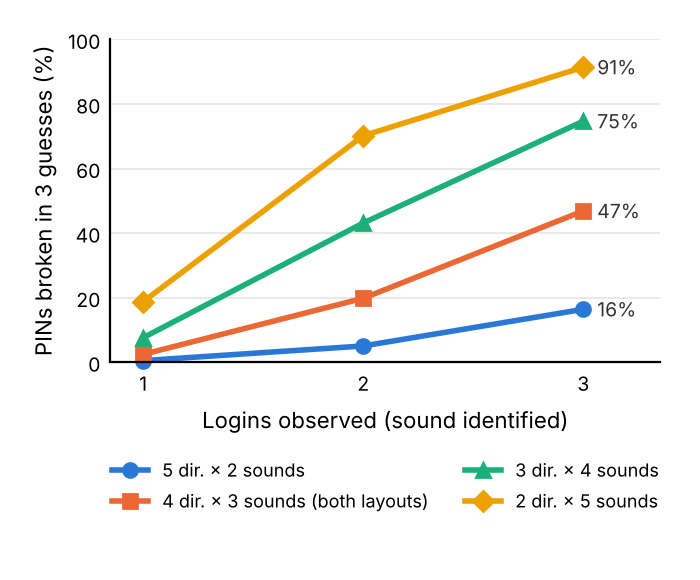
\includegraphics[width=0.92\columnwidth]{figures/attack_results.png}
\caption{PINs broken within three guesses when the attacker identifies every sound, by number of
logins observed. Both four-direction layouts coincide for this attacker.}
\label{fig:attack}
\end{figure}

Table~\ref{tab:attack} and Fig.~\ref{fig:attack} show three things. First, video alone never beats
chance, as (\ref{eq:uniform}) predicts. Second, every sound added to the chart helps an acoustic
attacker: after three logins, 16.4\% of PINs fall with two sounds but 91.4\% with five. Third, the
front--back confusion of generic HRTFs works in the user's favour: with side information, four side
positions give 18.8\% against 79.8\% for left/front/right/back. These are model results with perfect
identification, an upper bound; the real attacker's identification rates still have to be measured.

\subsection{Software validation}
An automated browser test drives both applications end to end and checks 47 behaviours, including
sound loading, completion of every login condition with correct taps, chart generation for every
layout, CSV export, hash-only PIN storage, lockout across reloads and offline caching. All pass.

\subsection{Pilot study}
We ran an informal pilot on 17--18 November 2026 with the AudioPIN Lock app on participants' own phones.
The app's usage log records, for every complete unlock attempt, the result, the total time and, per digit,
the response time and the number of cue repeats; by design it never records keys or taps. Five log files
(sessions A--E) held 35 attempts, 29 of them with two directions and five sounds (Table~\ref{tab:study}).
Tester IDs were not entered, so sessions cannot be matched to individual people.

Only 11 of 35 attempts (31\%) unlocked. Successful unlocks took a median of 15.0\,s (range 9.3--22.3\,s),
about 3.3\,s per digit; failed attempts took longer (median 19.2\,s). A digit needed 1.36 automatic cue
repeats on average, only 28\% of digits were answered before the first repeat, and the replay button was
never used. Success rose from 2 of 11 in the first three attempts of each session to 9 of 24 afterwards,
which suggests learning. Because keys and taps are not logged, the log cannot tell whether a failure came
from mishearing a sound, miscounting on the ring or a wrong PIN.

Five participants rated the key-code method on the System Usability Scale~\cite{brooke1996sus}
(Table~\ref{tab:sus}): 70.5\,$\pm$\,14.2 on average (median 70), around the commonly cited average of 68
and at the lower edge of the ``acceptable'' range of~\cite{bangor2008sus}. Two of the respondents are the authors; the other
three averaged 70.0\,$\pm$\,20.0. One respondent gave 5 to every item, including the negatively worded
ones; without that response the mean is 75.6\,$\pm$\,9.7. These are first-session numbers without a
normal-PIN baseline, and SSSL needed weeks of practice to reach its best times~\cite{perkovic2010sssl}.

\begin{table}[t]
\centering
\caption{Pilot unlock attempts logged by the AudioPIN Lock app, per session.}
\label{tab:study}
\setlength{\tabcolsep}{4pt}
\begin{tabular}{lcccc}
\toprule
Session & Layout(s) & Success / attempts & Rate & Time$^{*}$ (s) \\
\midrule
A & $2\times5$                  & 1 / 4   & 25\%  & 22.3 \\
B & $2\times5$                  & 1 / 9   & 11\%  & 12.9 \\
C & $2\times5$, $3\times4$, $4\times3$ & 7 / 20  & 35\%  & 16.0 \\
D & $2\times5$                  & 1 / 1   & 100\% & 13.7 \\
E & $2\times5$                  & 1 / 1   & 100\% & 9.3 \\
\midrule
All &                           & 11 / 35 & 31\%  & 15.0 \\
\bottomrule
\end{tabular}

\vspace{2pt}
{\footnotesize $^{*}$Median time of successful unlocks (all: range 9.3--22.3\,s).}
\end{table}

\begin{table}[t]
\centering
\caption{System Usability Scale (0--100) for the AudioPIN key-code method.}
\label{tab:sus}
\begin{tabular}{lcc}
\toprule
Respondents & $N$ & SUS, mean $\pm$ SD \\
\midrule
All                          & 5 & 70.5 $\pm$ 14.2 \\
Excluding the two authors    & 3 & 70.0 $\pm$ 20.0 \\
Excluding one straight-lined response & 4 & 75.6 $\pm$ 9.7 \\
\bottomrule
\end{tabular}
\end{table}

\subsection{Timing leak}
A digit $d$ wraps past 9 with probability $d/10$, and counting past the wrap may take longer, so a
stopwatch could hint at large digits~\cite{perkovic2010partially}. The lock app's log deliberately omits
keys and taps, so it cannot show which digits wrapped, and this pilot could not test the leak. The
research prototype records it per digit and will be used for that analysis.

% ------------------------------------------------------------------------------------- V
\section{Conclusion}
AudioPIN moves the per-digit secret of PIN entry from the screen to the earphones. A fresh uniform key
for every digit makes each tap equally likely, so recording the screen, once or many times, does not
help an attacker. The attack simulation shows where the remaining risk lies: a microphone that
identifies the sounds, a risk that falls as the layout uses more directions and fewer sounds. The pilot shows that unlocking takes about 15\,s and is rated
acceptable, but is not yet reliable: only 31\% of first-day attempts succeeded. The main limitations are this acoustic leak, the possible wrap-around
timing leak, front--back confusion with generic HRTFs, a small first-session pilot without a normal-PIN baseline or tester IDs, and the small
space of four-digit PINs; the lock app is an app lock, not a replacement for the operating system's.
Next, we will measure how well a real recording reveals sound and side, enforce a constant minimum time
per digit, and run a longer study.

% ------------------------------------------------------------------------------------- AI
\section*{AI Usage Declaration}
We used Claude (Anthropic) during this project. It reorganised the codebase into modules, wrote the
README, the automated browser test, the attack-simulation script (re-implemented from our threat model;
its results matched our earlier table) and the study-analysis script, set up this LaTeX template with
its tables and figures, computed the pilot statistics from our logs, checked the bibliography entries,
and rewrote the text of this report from our draft for structure and clarity. The method, the design
decisions, the choice of sounds and the user study are our own, and we checked every claim and number
in this report against the code and data.

\bibliographystyle{IEEEtran}
\bibliography{references}

\end{document}
